

%\blueheader
%\begin{frame}{2A: Snille funksjoner kan stykkevis tilnærmes med rette %linjer}
%\begin{figure}
%    \centering
%    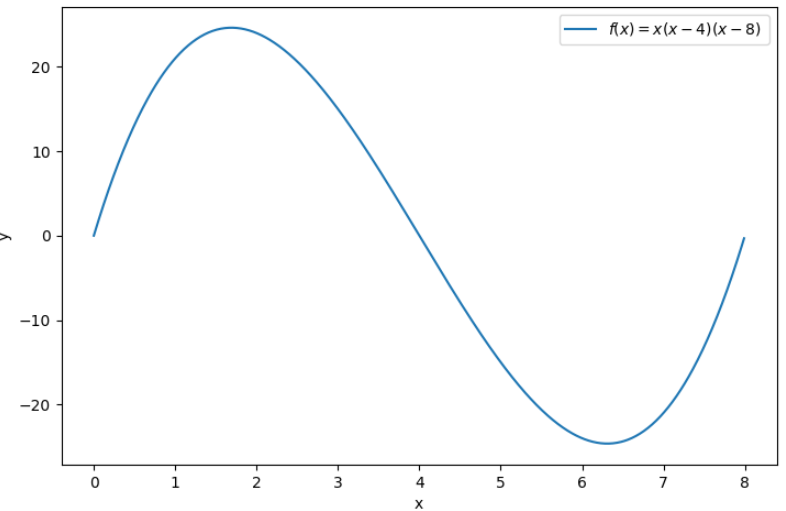
\includegraphics[width=0.8\linewidth]{R2-K2A-3.png}
%\end{figure}
%\end{frame}

\blueheader
\begin{frame}{2A: Det bestemte integralet}
\begin{figure}
    \centering
    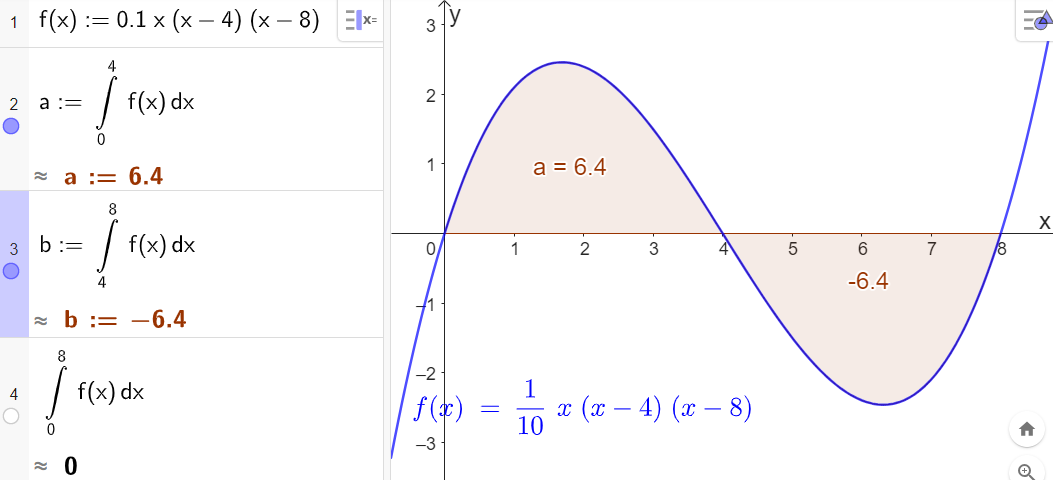
\includegraphics[width=\linewidth]{R2-K2A-1.png}
\end{figure}
\end{frame}

\blueheader
\begin{frame}{2A: Nedre trappesum, $N$}
\begin{figure}
    \centering
    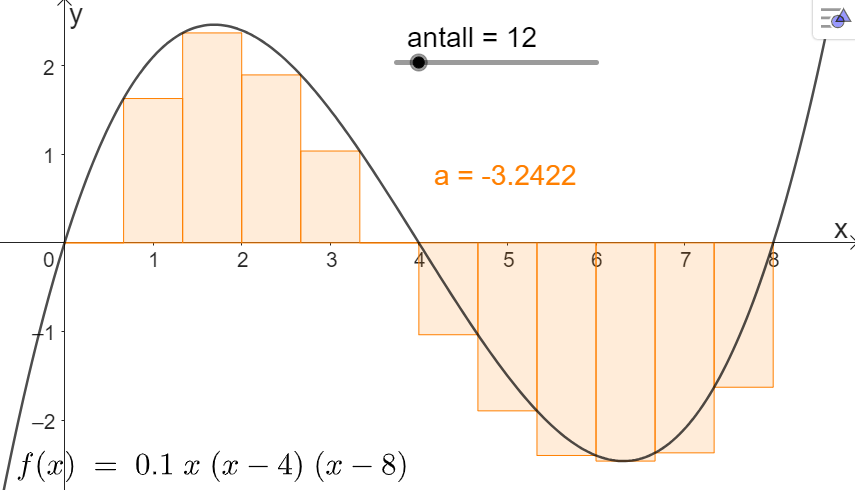
\includegraphics[width=0.7\linewidth]{R2-K2A-6.png}
\end{figure}

\href{https://www.geogebra.org/classic/rp6mbmm6}{Link til GeoGerba-fil}
\end{frame}

\blueheader
\begin{frame}{2A: Øvre trappesum, Ø}
\begin{figure}
    \centering
    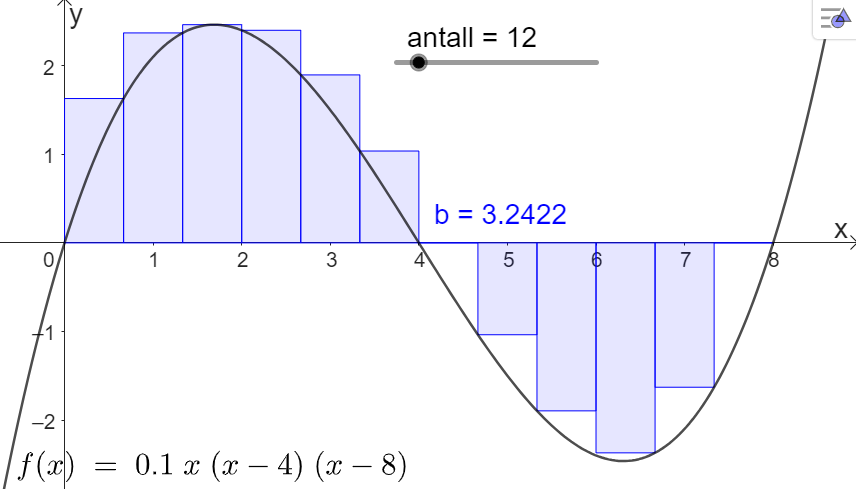
\includegraphics[width=0.7\linewidth]{R2-K2A-7.png}

\end{figure}

\href{https://www.geogebra.org/classic/rp6mbmm6}{Link til GeoGerba-fil}
\end{frame}

\blueheader
\begin{frame}{2A: Arealet må ligge mellom nedre og øvre trappesum. $N\leq A\leq$ Ø}
\begin{figure}
    \centering
    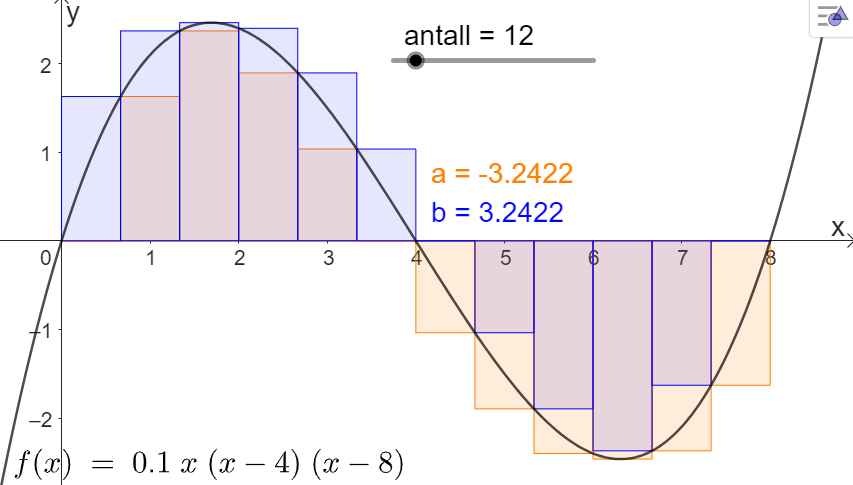
\includegraphics[width=0.7\linewidth]{R2-K2A-8.png}

\end{figure}

\href{https://www.geogebra.org/classic/rp6mbmm6}{Link til GeoGerba-fil}
\end{frame}

\blueheader
\begin{frame}{2A: Det bestemte integralet}

La  $\{N_n\}$ være tallfølgen av nedre trappesummer.

\medskip
La  $\{\text{Ø}_n\}$ være tallfølgen av nedre trappesummer  .

\medskip
Ideen bak definisjonen av det bestemte integralet, er at trappesummene blir bedre og bedre tilnærminger for arealet når antall rektangler går mot uendelig.

\begin{blue*}{Definisjonen av det bestemte integralet}
Det bestemte integralet som en grenseverdi til en følge av summer
\begin{equation*}
    \lim_{n\rightarrow \infty }N_ n =\lim_{n\rightarrow \infty }\text{Ø}_n=\int_a^bf(x)\;dx
\end{equation*}
Dersom grenseverdiene er forskjellige, er $f$ ikke integrerbar.
\end{blue*}
\end{frame}

\redheader
\begin{frame}{2A: Integrerbare funksjoner}
Hvis $f$ er en \textbf{kontinuerlig funksjon} på et intervall $[a,b]$ på x-aksen,  
så kan vi alltid regne ut \textbf{integralet} av $f$ på dette intervallet.  

\medskip

\[
    \int_a^b f(x)\,dx
\]

\medskip
\begin{itemize}
    \item Integral = ''arealet'' mellom grafen til $f$  
          og x-aksen i intervallet fra $x=a$ til $x=b$.
    \item ''Areal'' over x-aksen er positivt, og ''arealet'' under x-aksen er negativt.
\end{itemize}
\end{frame}

\blueheader
\begin{frame}[fragile]{2A: Integraler i GeoGebra: \texttt{integral(funksjon, start, slutt)}}
\begin{figure}
    \centering
    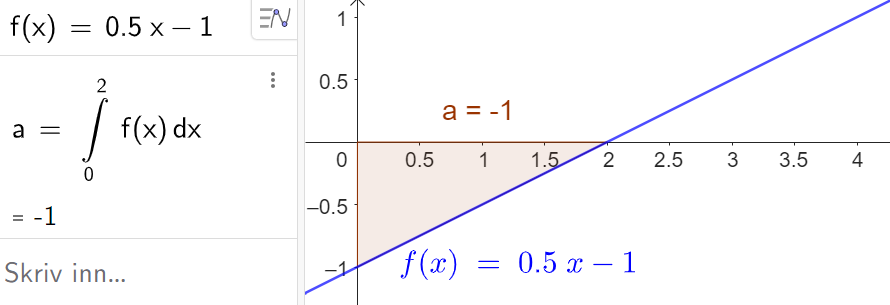
\includegraphics[width=\linewidth]{R2-K2A-9.png}
    \caption{\texttt{integral(0.5x-1, 0, 2)}}
\end{figure}
\end{frame}

\blueheader
\begin{frame}[fragile]{2A: Integraler i GeoGebra: \texttt{integral(funksjon, start, slutt)}}
\begin{figure}
    \centering
    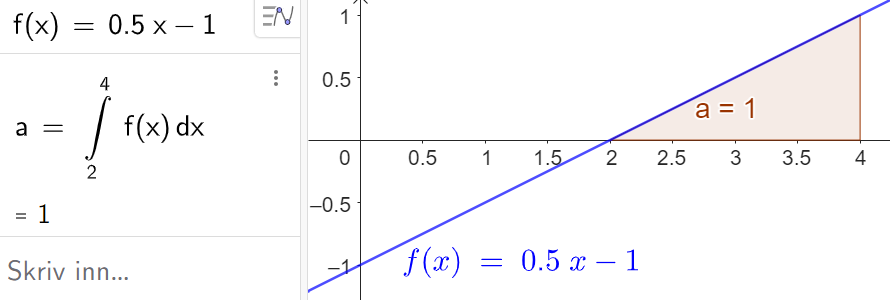
\includegraphics[width=\linewidth]{R2-K2A-10.png}
    \caption{\texttt{integral(0.5x-1, 2, 4)}}
\end{figure}
\end{frame}

\blueheader
\begin{frame}[fragile]{2A: Integraler i GeoGebra: \texttt{integral(funksjon, start, slutt)}}
\begin{figure}
    \centering
    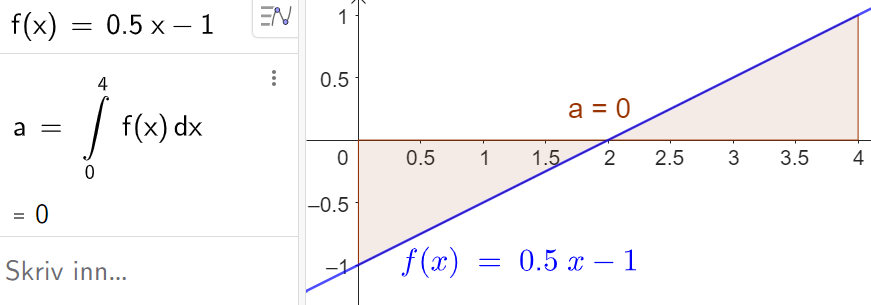
\includegraphics[width=\linewidth]{R2-K2A-11.png}
    \caption{\texttt{integral(0.5x-1, 0, 4)}}
\end{figure}
\end{frame}

\blueheader
\begin{frame}[fragile]{2A: Integraler i kombinasjon med \emph{Dersom} i CAS}
\begin{figure}
    \centering
    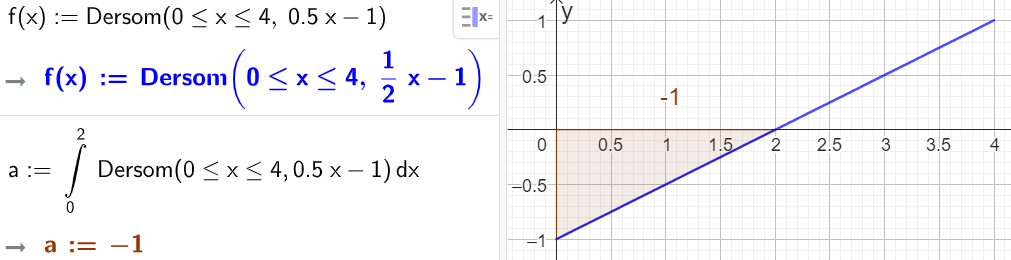
\includegraphics[width=\linewidth]{R2-K2A-13.png}
\end{figure}
\end{frame}

\blueheader
\begin{frame}[fragile]{2A: Integraler i kombinasjon med \emph{Løs} i CAS}
\begin{figure}
    \centering
    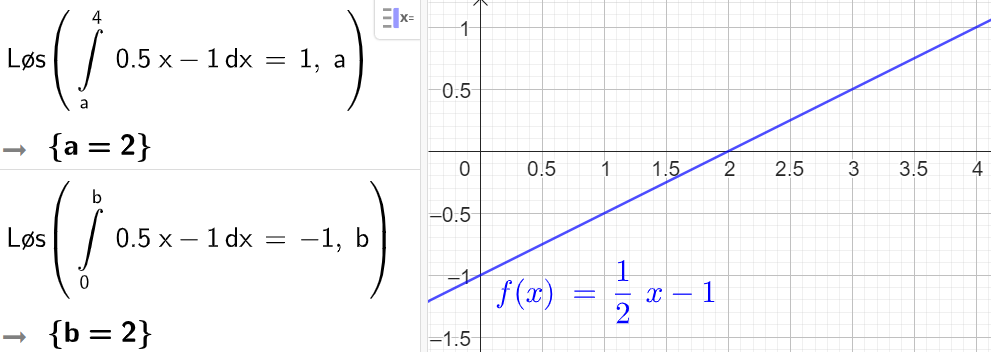
\includegraphics[width=\linewidth]{R2-K2A-12.png}
\end{figure}
\end{frame}

\greenheader
\begin{frame}[fragile]{2A: Integraler i Python hvis dere vil}
    \warn
\begin{figure}
    \centering
    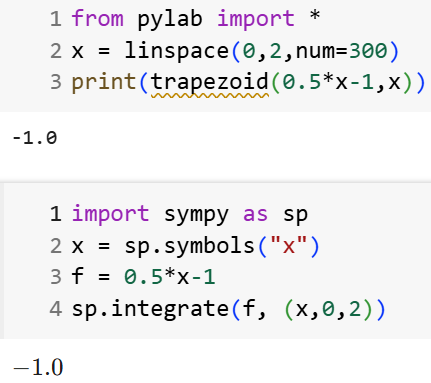
\includegraphics[width=0.5\linewidth]{R2-K2A-14.png}
\end{figure}
\end{frame}


\greenheader
\begin{frame}{2A: Uttrykk for nedre trappesum, $N_n$,  for en strengt voksende funksjon}
    \begin{columns} 
        \begin{column}{0.42\textwidth}
            Bredden av rektanglene på figuren er 
            \[
                \Delta x = \frac{b-a}{n}.
            \]
            Høyden i rektanglene er 
            \[
                f(x_0), f(x_1), f(x_2), \dots, f(x_{n-1}).
            \]
           
            
        \end{column}
        \begin{column}{0.58\textwidth}
            \centering
            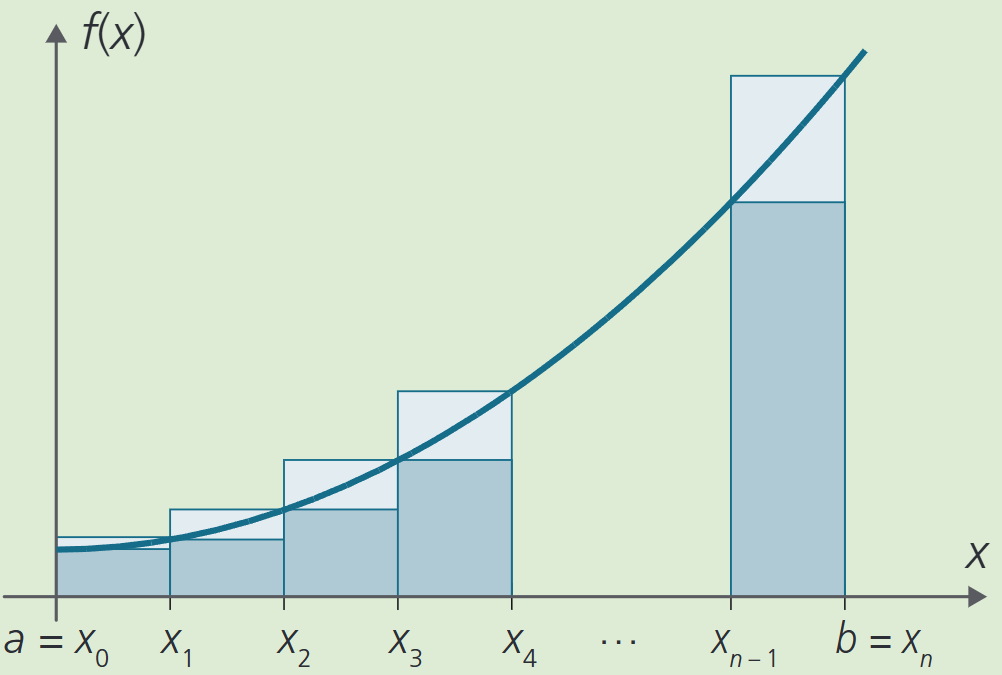
\includegraphics[width=1\linewidth]{R2-K2A-15.png}
        \end{column}
    \end{columns}
    \begin{align*}
                 N_n &=  
                 f(x_0)\cdot \Delta x + f(x_1)\cdot \Delta x + f(x_2)\cdot \Delta x \dots + f(x_{n-1})\cdot \Delta x\\
                &=  \sum_{i=1}^{n} f(x_{i-1})\cdot \Delta x
            \end{align*}
\end{frame}

\greenheader
\begin{frame}{2A: Uttrykk for øvre trappesum $\text{Ø}_n$,  for en strengt voksende funksjon}
    \begin{columns} 
        \begin{column}{0.42\textwidth}
            Bredden av rektanglene på figuren er 
            \[
                \Delta x = \frac{b-a}{n}.
            \]
            Høyden i rektanglene er 
            \[
                f(x_1), f(x_2), f(x_3), \dots, f(x_{n}).
            \]
           
            
        \end{column}
        \begin{column}{0.58\textwidth}
            \centering
            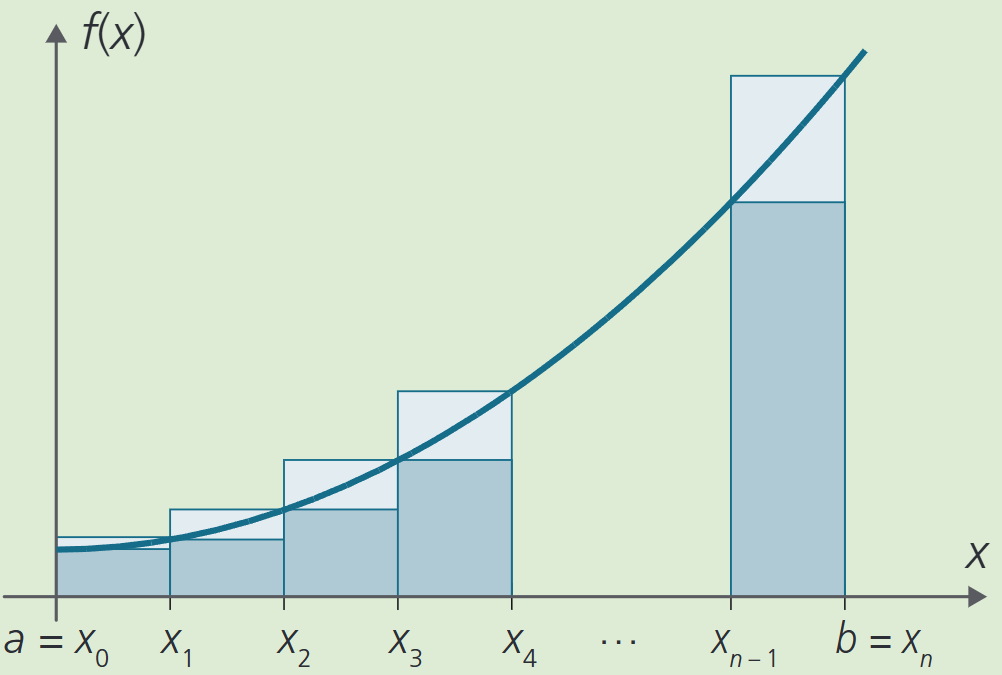
\includegraphics[width=1\linewidth]{R2-K2A-15.png}
        \end{column}
    \end{columns}
    \begin{align*}
                 \text{Ø}_n &=  
                 f(x_1)\cdot \Delta x + f(x_2)\cdot \Delta x + f(x_3)\cdot \Delta x \dots + f(x_{n})\cdot \Delta x\\
                &=  \sum_{i=1}^{n} f(x_{i})\cdot \Delta x
            \end{align*}
\end{frame}

\blueheader
\begin{frame}{2A: Nedre trappesum til en funksjon som ikke er strengt voksende}
Merk at generelt tar 
\begin{itemize}
    \item nedre trappesum utgangspunkt i den minste høyden til rektanglet.\\
    \item og øvre trappesum tar utgangspunkt i den største høyden til rektanglet.
\end{itemize}
\begin{figure}
    \centering
    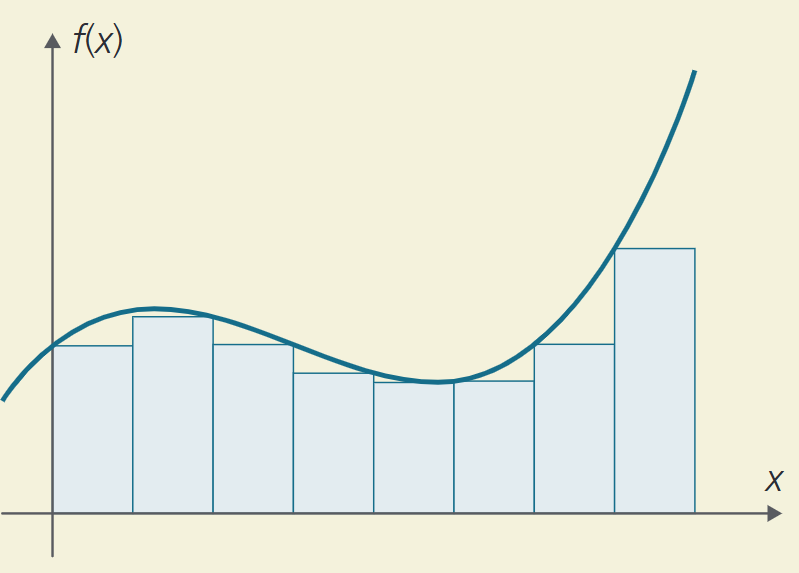
\includegraphics[width=0.6\linewidth]{R2-K2A-17.png}
\end{figure}
\end{frame}

\blueheader
\begin{frame}{2A: Venstre- og høyre-tilnærming}
\begin{figure}
    \centering
    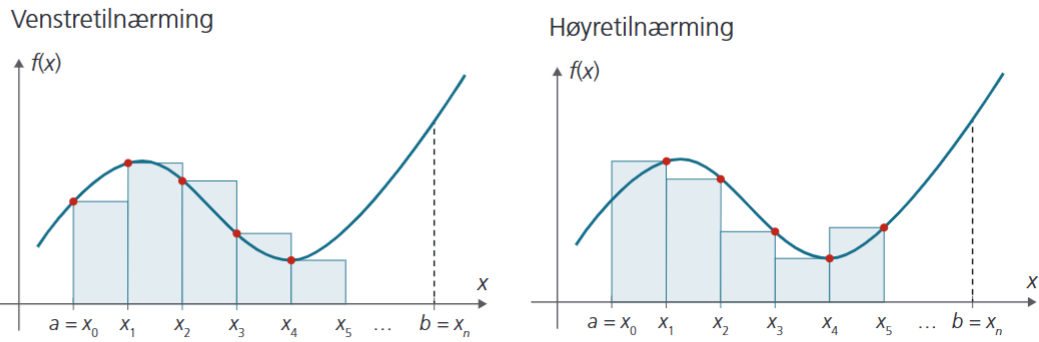
\includegraphics[width=\linewidth]{R2-K2B-2.png}
\end{figure}
\end{frame}





